
%(BEGIN_QUESTION)
% Copyright 2014, Tony R. Kuphaldt, released under the Creative Commons Attribution License (v 1.0)
% This means you may do almost anything with this work of mine, so long as you give me proper credit

Anta at tre ulike voltmetre er koblet til et termoelement, der hvert voltmeter har ulik omgivelsestemperatur:

$$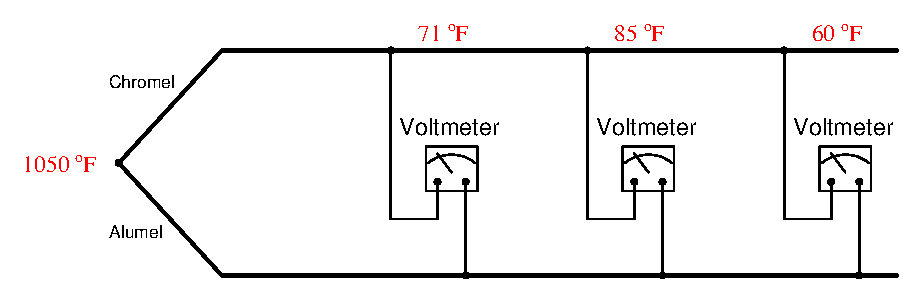
\includegraphics[width=15.5cm]{i00873x01.eps}$$

Beregn spenningen registrert av hvert av de tre voltmetrene, og svar på følgende spørsmål:

\begin{itemize}
\item{} Hvis et fjerde voltmeter kobles til samme termoelement, vil det påvirke målingene til de tre andre?
\vskip 5pt
\item{} Hvis en termoelementtransmitter kobles til dette termoelementet, vil det påvirke voltmeteravlesningene? Vil det ha betydning om transmitteren har referansekrysskompensasjon eller ikke?
\end{itemize}

\underbar{file i00873}
%(END_QUESTION)





%(BEGIN_ANSWER)

Hvert voltmeter danner sitt eget referansekryss der kobberledningene i voltmeteret kobles til kromel- og alumel-lederne i termoelementet. Hvert referansekryss genererer sin egen spenning med motsatt polaritet av målekryssets spenning (ved 1050 $^{o}$F). Derfor må vi gjøre separat spenningsberegning for hvert voltmeter basert på meterets referansekrysstemperatur. Ekvivalentskjemaet viser hvordan de fire metallovergangene henger sammen med de tre voltmetrene:

$$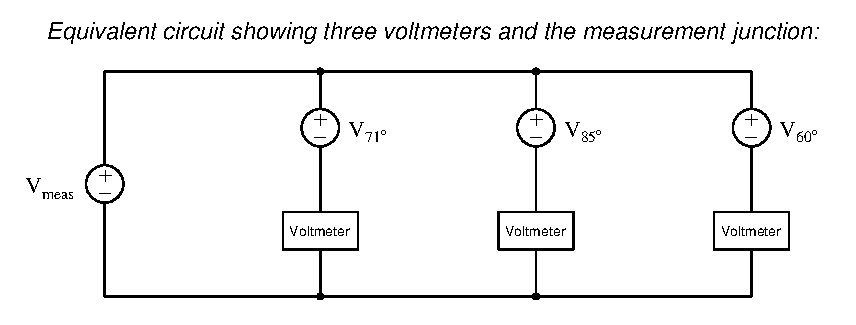
\includegraphics[width=15.5cm]{i00873x02.eps}$$

Kromel og alumel identifiserer dette som et {\bf type K}-termoelement, og vi kan bruke type K-tabell for å finne spenningene ved de fire krysstemperaturene:

\begin{itemize}
\item{} Type K ved 1050 $^{o}$F = 23.439 mV
\item{} Type K ved 71 $^{o}$F = 0.865 mV
\item{} Type K ved 85 $^{o}$F = 1.181 mV
\item{} Type K ved 60 $^{o}$F = 0.619 mV
\end{itemize}

\vskip 10pt

Siden målekryss og referansekryss står mot hverandre i hver voltmeterløkke, finner vi hver avlesning ved å trekke referansekryss-spenningen fra målekryss-spenningen:

\vskip 10pt

\noindent
{\bf Spenning registrert av venstre voltmeter (ved 71 $^{o}$F):}

$$23.439 \hbox{ mV} - 0.865 \hbox{ mV} = 22.574 \hbox{ mV}$$

\vskip 10pt

\noindent
{\bf Spenning registrert av midterste voltmeter (ved 85 $^{o}$F):}

$$23.439 \hbox{ mV} - 1.181 \hbox{ mV} = 22.258 \hbox{ mV}$$

\vskip 10pt

\noindent
{\bf Spenning registrert av høyre voltmeter (ved 60 $^{o}$F):}

$$23.439 \hbox{ mV} - 0.619 \hbox{ mV} = 22.820 \hbox{ mV}$$

\vskip 10pt

Spenningen hvert voltmeter leser er en direkte følge av Kirchhoffs spenningslov, der målekrysset og meterets referansekryss er de eneste spenningskildene i KVL-løkken. Derfor vil tilkobling av et fjerde voltmeter ikke påvirke de tre andre. Tilsvarende vil tilkobling av en termoelementtransmitter til samme kromel/alumel-ledningspar ikke påvirke voltmeteravlesningene, verken med eller uten referansekrysskompensasjon.

%(END_ANSWER)





%(BEGIN_NOTES)


%INDEX% Measurement, temperature: thermocouple

%(END_NOTES)
